It is well known that polynomial smoothers allow more aggressive coarsening than Jacobi \cite{brannick2015polynomial}.
For further discussion of the error propagation properties of the Chebyshev semi-iterative method, see \cite{gutknecht2002revisited}.

We use the Jacobi preconditioned operator, $\left( \diag {\color{burgundy}\mathbf{A}} \right)^{-1} {\color{burgundy}\mathbf{A}}$, in this iteration instead of the finite element operator ${\color{burgundy}\mathbf{A}}$, similar to the discussion in \cite{adams2003parallel}.

The terms in the Chebyshev semi-iterative method can be modeled by the three term recurrence relation given by
\begin{equation}
\mathbf{u}_{k + 1} = - \left( \mathbf{r}_k + \alpha \mathbf{u}_k + \beta_{k - 1} \mathbf{u}_{k - 1} \right) / \gamma_{k - 1}
\label{eq:chebyshev_recursive}
\end{equation}
where the spectrum of $\left( \diag {\color{burgundy}\mathbf{A}} \right)^{-1} {\color{burgundy}\mathbf{A}}$ lies on the line segment $\left[ \alpha - c, \alpha + c \right]$ and the parameters $\beta$ and $\gamma$ are given by the recurrence
\begin{equation}
\begin{tabular}{c c}
$\beta_0 = - \frac{c^2}{2 \alpha}$ & $\gamma_0 = - \alpha$\\
$\beta_k = \frac{c}{2} \frac{T_k \left( \eta \right)}{T_{k + 1} \left( \eta \right)} = \left( \frac{c}{2} \right)^2 \frac{1}{\gamma_k}$ & $\gamma_k = \frac{c}{2} \frac{T_{k + 1} \left( \eta \right)}{T_k \left( \eta \right)} = - \left( \alpha + \beta_{k - 1} \right)$.
\end{tabular}
\end{equation}
In this equation, $T_i \left( \zeta \right) = 2 \zeta T_{i - 1} \left( \zeta \right) - T_{i - 2} \left( \zeta \right)$ are the classical Chebyshev polynomials, which are evaluated at the point $\eta = - \alpha / c$.

The residual in the Chebyshev semi-iterative method can therefore be modeled by the three term recurrence
\begin{equation}
\mathbf{r}_k = \left( \left( \diag {\color{burgundy}\mathbf{A}} \right)^{-1} {\color{burgundy}\mathbf{A}} \mathbf{r}_{k - 1} - \alpha \mathbf{r}_{k - 1} - \beta_{k - 2} \mathbf{r}_{k - 2} \right) / \gamma_{k - 1}.
\label{eq:chebyshev_error_recursive}
\end{equation}

Using the recurrence relation given in Equation \ref{eq:chebyshev_error_recursive}, we can define the error propagation of the $k$th order Chebyshev smoother in terms of the error in the first term:
\begin{equation}
\begin{tabular}{c}
$\mathbf{E}_0 = \mathbf{I}$\\
$\mathbf{E}_1 = \mathbf{I} - \frac{1}{\alpha} \left( \diag {\color{burgundy}\mathbf{A}} \right)^{-1} {\color{burgundy}\mathbf{A}}$\\
$\mathbf{E}_k = \left( \left( \diag {\color{burgundy}\mathbf{A}} \right)^{-1} {\color{burgundy}\mathbf{A}} \mathbf{E}_{k - 2} - \alpha \mathbf{E}_{k - 1} - \beta_{k - 2} \mathbf{E}_{k - 2} \right) / \gamma_{k - 1}$
\end{tabular}
\label{eq:chebyshev_error_propagation}
\end{equation}
With this recursive definition of the error propagation operator, we can define the symbol for Chebyshev smoothing.

\begin{definition}
The symbol of the error propagation operator for $k$th order Chebyshev smoothing based on the Jacobi preconditioned operator is given by
\begin{equation}
\tilde{\mathbf{S}} \left( \nu, n, \boldsymbol{\theta} \right) = \left( \tilde{\mathbf{E}}_k \right)^\nu,
\end{equation}
where $\nu$ is the number of smoothing passes and $\tilde{\mathbf{E}}_k \left( \boldsymbol{\theta} \right)$ is given by the recursive definition
\begin{equation}
\begin{tabular}{c}
$\tilde{\mathbf{E}}_0 \left( \boldsymbol{\theta} \right) = \mathbf{I}$\\
$\tilde{\mathbf{E}}_1 \left( \boldsymbol{\theta} \right) = \mathbf{I} - \frac{1}{\alpha} \tilde{\color{burgundy}\mathbf{A}}_J \tilde{\color{burgundy}\mathbf{A}} \left( \boldsymbol{\theta} \right)$\\
$\tilde{\mathbf{E}}_k \left( \boldsymbol{\theta} \right) = \left( \tilde{\color{burgundy}\mathbf{A}}_J \tilde{\color{burgundy}\mathbf{A}} \left( \boldsymbol{\theta} \right) \tilde{\mathbf{E}}_{k - 2} \left( \boldsymbol{\theta} \right) - \alpha \tilde{\mathbf{E}}_{k - 1} \left( \boldsymbol{\theta} \right) - \beta_{k - 2} \tilde{\mathbf{E}}_{k - 2} \left( \boldsymbol{\theta} \right) \right) / \gamma_{k - 1}$
\end{tabular}
\end{equation}
\label{def:chebyshev_symbol}
\end{definition}
with $\tilde{\color{burgundy}\mathbf{A}}_J = \left( \mathbf{Q}^T \diag \left( {\color{burgundy}\mathbf{A}}^e \right) \mathbf{Q} \right)^{-1}$ giving the symbol of the Jacobi smoother.

\begin{figure}[!ht]
  \centering
  \subfloat[Spectrum of 1D Chebyshev for $p = 4$]{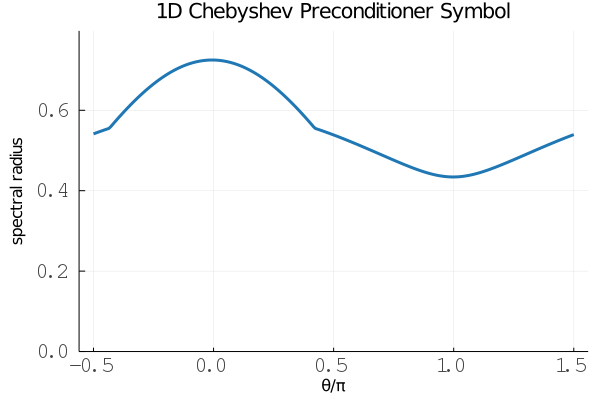
\includegraphics[width=0.48\textwidth]{../img/ChebyshevSymbol1D}\label{fig:chebyshev_spectrum_1d}}
  \hfill
  \subfloat[Spectrum of 2D Chebyshev for $p = 4$]{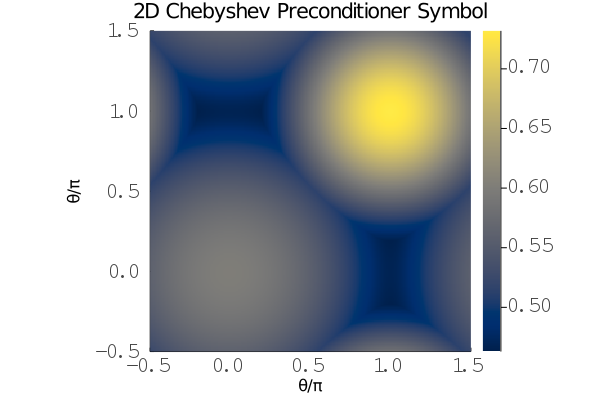
\includegraphics[width=0.48\textwidth]{../img/ChebyshevSymbol2D}\label{fig:chebyshev_spectrum_2d}}
  \caption{Spectrum of Chebyshev Preconditioner Symbol}
\end{figure}

Using Definition \ref{def:chebyshev_symbol}, in Figures \ref{fig:chebyshev_spectrum_1d} and \ref{fig:chebyshev_spectrum_2d}, we see the spectral radius of the symbol of third order Chebyshev polynomial preconditioning for the scalar diffusion operator with a fourth-order H1 Lagrange finite element basis on the Gauss-Lobatto points in one and two dimensions.
When compared to Figures \ref{fig:jacobi_spectrum_1d} and \ref{fig:jacobi_spectrum_2d}, we can see that smoothing based upon Chebyshev semi-iterative offers better error reduction than weighted or unweighted Jacobi, albeit at a higher computational cost.
